\chapter{Experimentació i resultats}
\label{cap:resultados}

Un TFM d'enginyeria cau si aquest capítol és només una galeria de captures. Cal declarar \emph{què} es mesura, \emph{com} es reprodueix i \emph{què} no s'afirma. Aquí ``resultat'' vol dir evidència reproduïble, no una impressió (``el xat funciona bé'').

\section{Preguntes d'avaluació}

Les preguntes segueixen el cicle del capítol~\ref{cap:intro} i els requisits del~\ref{cap:requisitos}:

\begin{enumerate}[label=E\arabic*.]
  \item El pipeline indexa un PDF de text i deixa el document en estat llest? (RF-03)
  \item La recuperació híbrida retorna $k>0$ chunks en una assignatura amb corpus conegut?
  \item Quina és la latència p50/max del retrieval (embedding + híbrid) en aquest corpus?
  \item Els tests automàtics del repositori es mantenen verds?
  \item El cicle UI (documents llestos $\rightarrow$ xat amb cita $\rightarrow$ qüestionari $\rightarrow$ planner) es pot executar? (RF-05 a RF-10)
\end{enumerate}

\paragraph{Què és p50.}
El percentil 50 (mediana) de latència: la meitat de les consultes acaben en aquest temps o menys. Es prefereix a la mitjana perquè una consulta lenta no desplaça tot el resum. El \texttt{max} documenta el pitjor cas observat, no un SLA.

\paragraph{Què no es mesura.}
La \emph{groundedness} (si cada frase de la resposta està suportada per un chunk) exigiria un protocol d'anotació o un jutge LLM; no es reporta com a mètrica tancada. Tampoc: durada d'ingestió (parse + embeddings), latència extrem a extrem del xat (retrieval + LLM + SSE), precisió del classificador d'intent, rellevància del top-$k$, ni un judici de la qualitat de les cartes o del qüestionari generats. Un estudi d'aprenentatge ($n$ alumnes, pre/post) queda fora d'abast. Afirmar-ho sense dades inflaria el capítol.

\section{Mètode}

\subsection{Qualitat de programari (sempre reproduïble)}

Al backend: tests unitaris, ruff i mypy. Al frontend: comprovació de tipus, Vitest i smoke Playwright (contra l'app en marxa).
Aquestes ordres, tret de Playwright, no depenen d'OpenAI. Playwright comprova que landing i login renderitzen; no executa el RAG.

\subsection{Recuperació (corpus real)}

El CLI de benchmark (annex~\ref{anexo:eval}) mesura durada i nombre de chunks retornats. El harness unitari només comprova que l'agregació (p50, max) no està trencada.

\paragraph{Corpus i consultes (31 d'agost de 2026).}
Una assignatura d'apunts reals cursada per l'autor (\emph{Direcció d'empreses tecnològiques i emprenedoria}), 114 chunks indexats. El PDF original no s'adjunta; a les captures, el contacte del professor del fragment està tapat. Vuit consultes \emph{factuals} (paraules del temari), repetides en els dos runs: \emph{modelo de negocio}, \emph{propuesta de valor}, \emph{lienzo canvas}, \emph{startup}, \emph{innovacion}, \emph{financiacion}, \emph{mercado objetivo}, \emph{equipo fundador}. El CLI executa cerca híbrida (densa + lèxica + RRF); no exposa una política ``només dens''. El segon run activa el rerank LLM sobre el mateix híbrid. No s'anota rellevància del top-5: només latència i $k$ retornat.

Aquestes vuit consultes no exerciten els intents de \emph{resum} ni de \emph{capítol} del capítol~\ref{cap:arquitectura}. El classificador i el filtre per número al nom de fitxer tenen tests unitaris; a la UI, el resum es veu a la figura~\ref{fig:ui-chat} i la nomenclatura dels PDF a la figura~\ref{fig:ui-docs}. No hi ha p50 d'aquests dos intents.

\subsection{Integració real}

Un test d'integració opt-in cobreix assignatura, pujada, ingestió i un xat mínim contra Supabase i l'LLM. No forma part de la CI (quota, no-determinisme, projecte que es pot pausar); l'ordre és a l'annex~\ref{anexo:eval}.

\section{Resultats de qualitat de programari}

\begin{table}[htbp]
\centering
\caption{Execució local de qualitat (backend 1/09/2026; frontend 31/08/2026).}
\label{tab:calidad}
\begin{tabular}{lll}
\toprule
Ordre & Resultat & Data \\
\midrule
\texttt{pytest tests/unit} & 63 passed (5,58\,s) & 01/09/2026 \\
\texttt{ruff check app tests} & sense errors & 01/09/2026 \\
\texttt{mypy app} & 77 fitxers, sense issues & 01/09/2026 \\
\texttt{tsc --noEmit} & OK & 31/08/2026 \\
Vitest & 4 tests, 2 fitxers & 31/08/2026 \\
Playwright smoke & 2 passed (1,3\,s), Chromium & 31/08/2026 \\
\bottomrule
\end{tabular}
\end{table}

E4 queda cobert. Els 4 tests Vitest cobren utilitats i contractes de client, no cada pantalla. Playwright comprova que landing i login renderitzen; \textbf{no} executa xat, quiz ni planner. El smoke \textbf{sí} corre a la CI del frontend (Chromium després del build, sense OpenAI). E5, doncs, no està automatitzat: el cicle d'estudi a la UI el demostren les captures autenticades de la secció~\ref{sec:cicle-ui}, no un E2E del RAG. E1 i E2 tenen cobertura unitària amb fakes; E1 també es veu a la UI (documents en estat \emph{Listo}, figura~\ref{fig:ui-docs}).

\section{Resultats de retrieval}

La taula~\ref{tab:bench} és el CLI sobre el corpus anterior, no un microbenchmark sintètic. Cada cas fa embedding de la consulta + \texttt{hybrid\_search}. El \texttt{max} de l'híbrid (3\,991\,ms) és la \emph{primera} consulta: arrencada en fred del client d'embeddings. El run amb rerank es va fer a continuació (model ja calent); el seu \texttt{max} no es pot llegir com a ``el rerank és més ràpid en el pitjor cas''. El que sí es compara és el p50: híbrid 369\,ms vs híbrid+rerank LLM 1\,608\,ms.

\paragraph{$k=10$ a la taula, $k=8$ al producte.}
El 31/08 el CLI (i el xat) cridaven \texttt{hybrid\_search} sense passar $k$: el defecte del port era \texttt{match\_count=10}. Per això la mitjana de chunks és 10,0. El valor de configuració \texttt{RETRIEVAL\_FINAL\_TOP\_K} (i el que documenta el capítol~\ref{cap:arquitectura} per al prompt) és 8. No són la mateixa $k$: la taula mesura latència a $k=10$, no un contrast de mida de context. El port, a l'estat actual, si s'omet $k$ aplica el 8 de la configuració.

La part de latència d'aquest corpus queda \emph{documentada} amb aquestes xifres; O6, com a objectiu d'avaluació, resta parcial (capítols~\ref{cap:intro} i~\ref{cap:conclusiones}). Resta obert el contrast ``només dens'' (el CLI no l'implementa) i qualsevol judici de rellevància o groundedness.

\begin{table}[htbp]
\centering
\caption{Benchmark de recuperació (8 consultes factuals, 114 chunks, $k=10$ al CLI d'aquest run, 31/08/2026).}
\label{tab:bench}
\begin{tabular}{lrrrr}
\toprule
Política & n consultes & p50 (ms) & max (ms) & mitjana chunks \\
\midrule
Híbrid (RRF) & 8 & 369 & 3991 & 10,0 \\
Híbrid + rerank LLM & 8 & 1608 & 2745 & 10,0 \\
\bottomrule
\end{tabular}
\end{table}

\section{Resultats qualitatius (cicle d'estudi)}
\label{sec:cicle-ui}

Les figures~\ref{fig:ui-docs}--\ref{fig:ui-planner} són captures de l'app en Docker (31/08/2026), sessió autenticada, mateixa assignatura del benchmark. A la barra es veu una assignatura auxiliar anomenada \emph{test}, fora del corpus mesurat. El correu de sessió al peu de la barra està tapat; a la figura~\ref{fig:ui-chat} també el contacte del professor que apareix al fragment indexat. \textbf{No substitueixen E3} (latència) ni un E2E automatitzat: \textbf{demostren E5} com a recorregut observable. El peu nomena el requisit, no l'estètica.

La taula~\ref{tab:intents-eval} lliga els tres intents del capítol~\ref{cap:arquitectura} amb l'evidència d'aquest capítol. El p50 només cobreix l'intent factual.

\begin{table}[htbp]
\centering
\caption{Intents del RAG i on es veuen en aquesta avaluació. Sense anotació de rellevància.}
\label{tab:intents-eval}
\small
\begin{tabularx}{\textwidth}{l >{\raggedright\arraybackslash}X >{\raggedright\arraybackslash}X}
\toprule
Intent & Evidència & Què no afirma \\
\midrule
Factual & 8 paraules clau al CLI (taula~\ref{tab:bench}) & Rellevància del top-$k$. \\
Resum & Figura~\ref{fig:ui-chat}: «Resume el tema en una frase.» & p50 ni fidelitat de la frase. \\
Capítol & Tests unitaris del classificador i del filtre per número al nom; PDF numerats a la figura~\ref{fig:ui-docs} (\texttt{3\_\ldots} $=$ tema~3) & No hi ha consulta cronometrada «explica el tema~3» a la UI. \\
\bottomrule
\end{tabularx}
\end{table}

\begin{figure}[htbp]
\centering
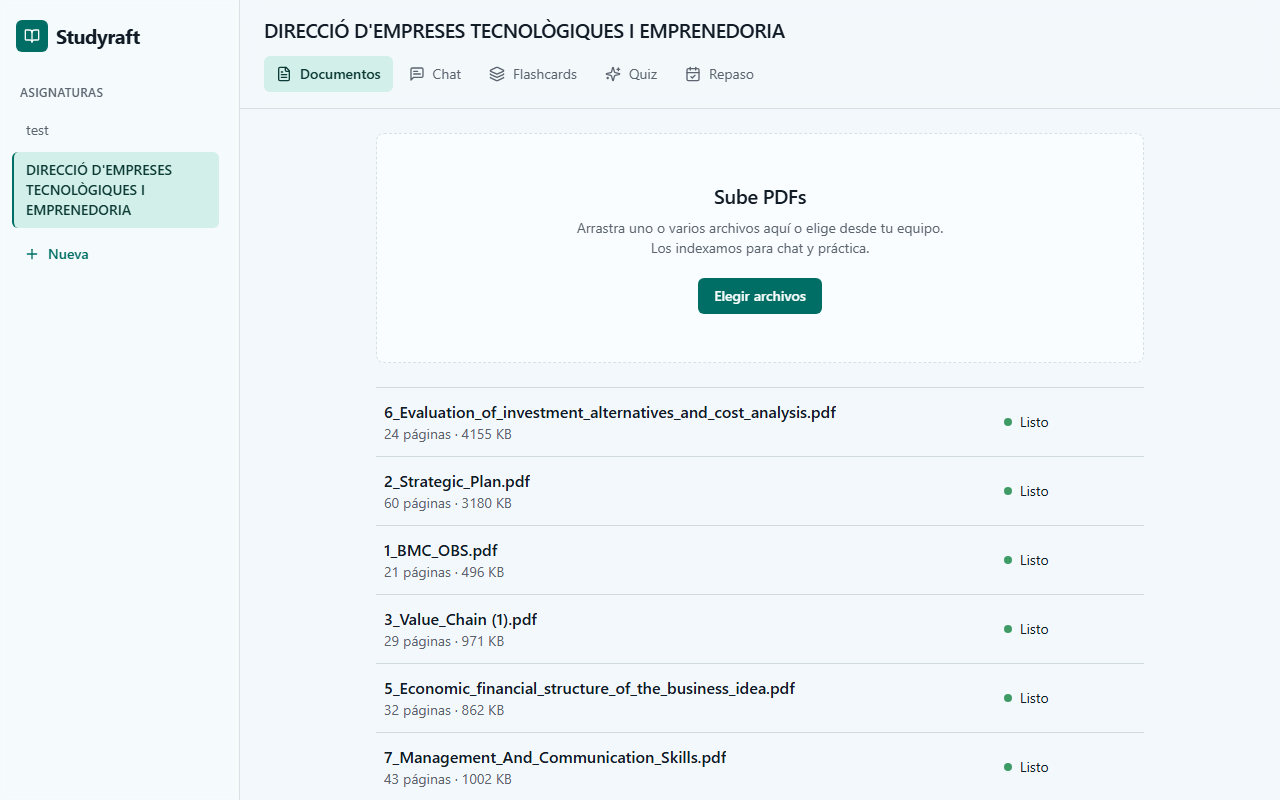
\includegraphics[width=0.92\textwidth]{figures/screenshots/04-documents.png}
\caption{Documents indexats en estat \emph{Listo} (RF-03). PDF de tema amb nom numerat (la llista es desplaça; el xat i el quiz en mostren vuit).}
\label{fig:ui-docs}
\end{figure}

\begin{figure}[htbp]
\centering
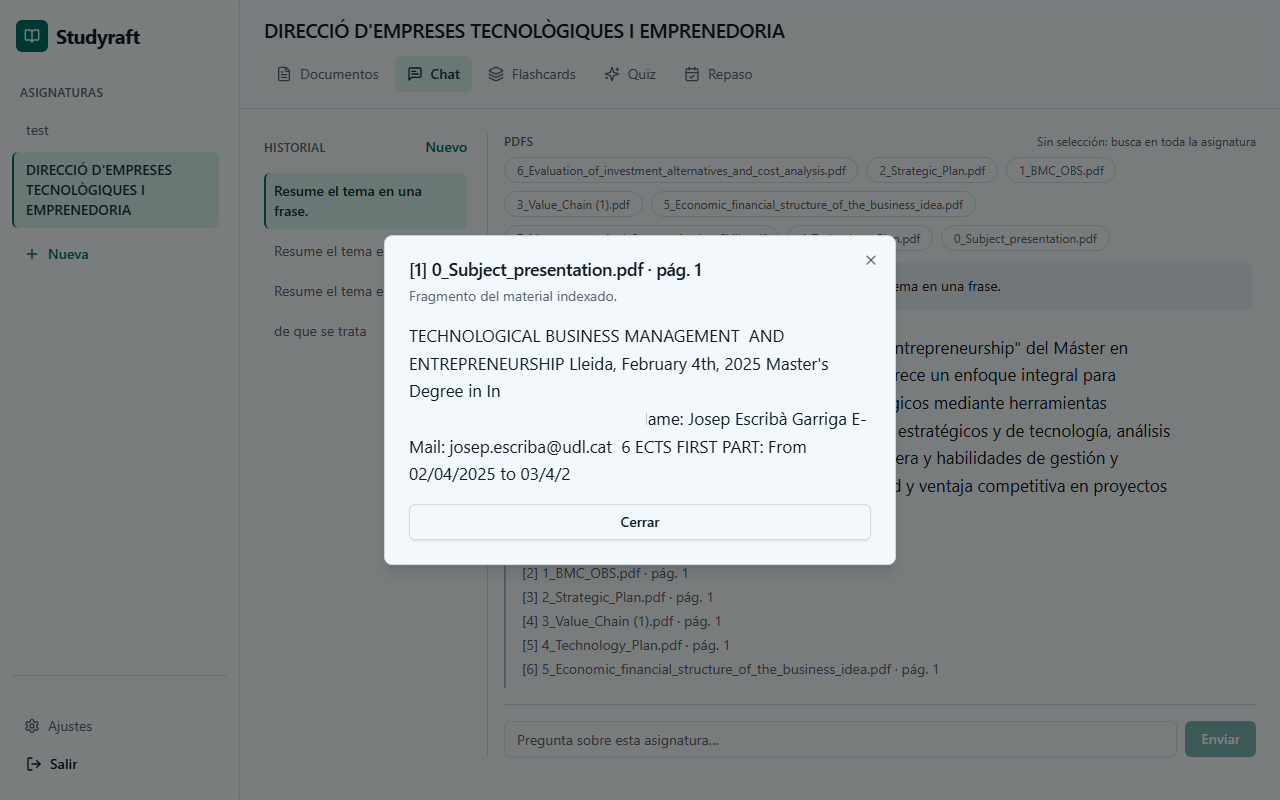
\includegraphics[width=0.92\textwidth]{figures/screenshots/05-chat.png}
\caption{Xat amb cita oberta: fitxer, pàgina i fragment indexat (RF-05 / RF-06). Correu de sessió i contacte del fragment, tapats.}
\label{fig:ui-chat}
\end{figure}

\paragraph{Recorregut de la figura~\ref{fig:ui-chat}.}
L'estudiant escriu «Resume el tema en una frase.»: intent \emph{resum} (capítol~\ref{sec:rag-pregunta}), sense filtre a un sol PDF. La resposta va en castellà de tu, ancorada al temari. La cita~\texttt{[1]} obre el fragment de \texttt{0\_Subject\_presentation.pdf}, pàgina~1 (presentació de l'assignatura). Això mostra el camí pregunta $\rightarrow$ intent $\rightarrow$ chunk citat; no mesura si cada oració de la resposta està al chunk.

\begin{figure}[htbp]
\centering
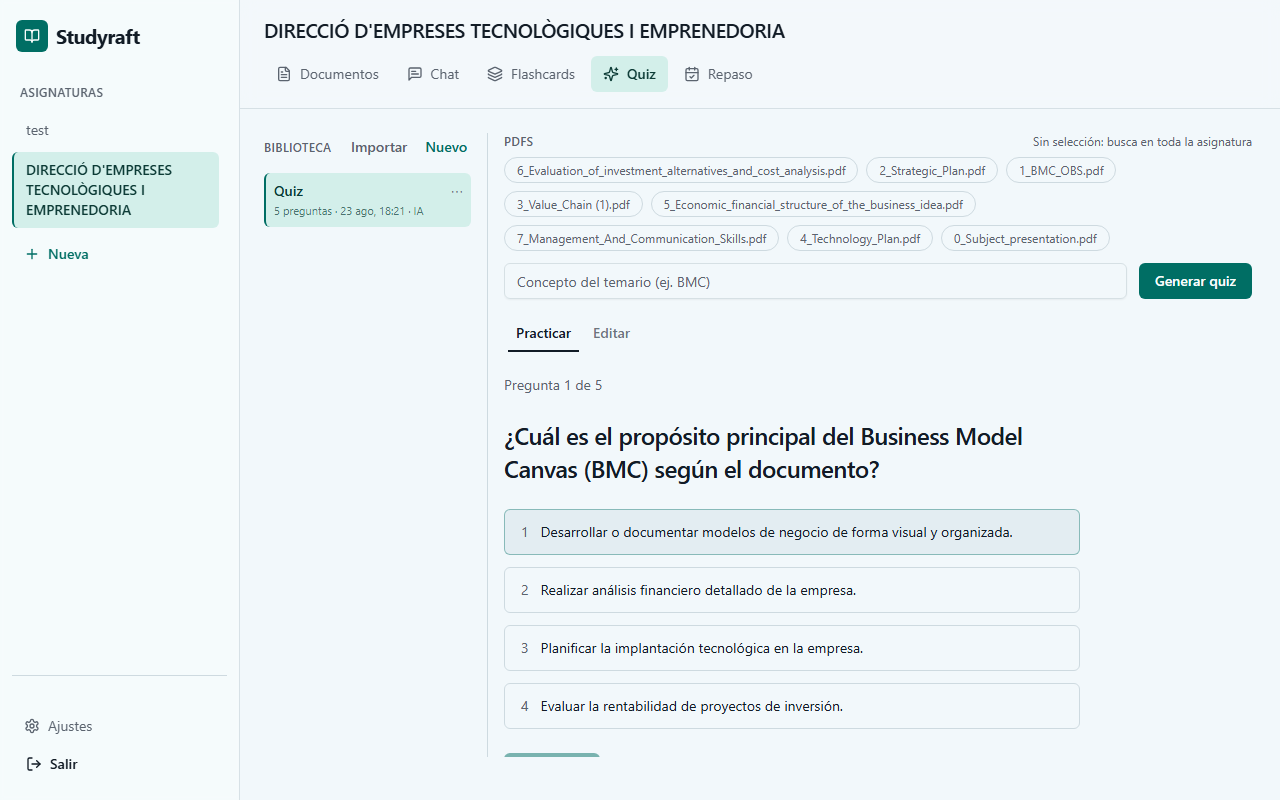
\includegraphics[width=0.92\textwidth]{figures/screenshots/06-quiz.png}
\caption{Qüestionari de pràctica generat sobre el corpus (RF-07): pregunta sobre el BMC, quatre opcions.}
\label{fig:ui-quiz}
\end{figure}

\begin{figure}[htbp]
\centering
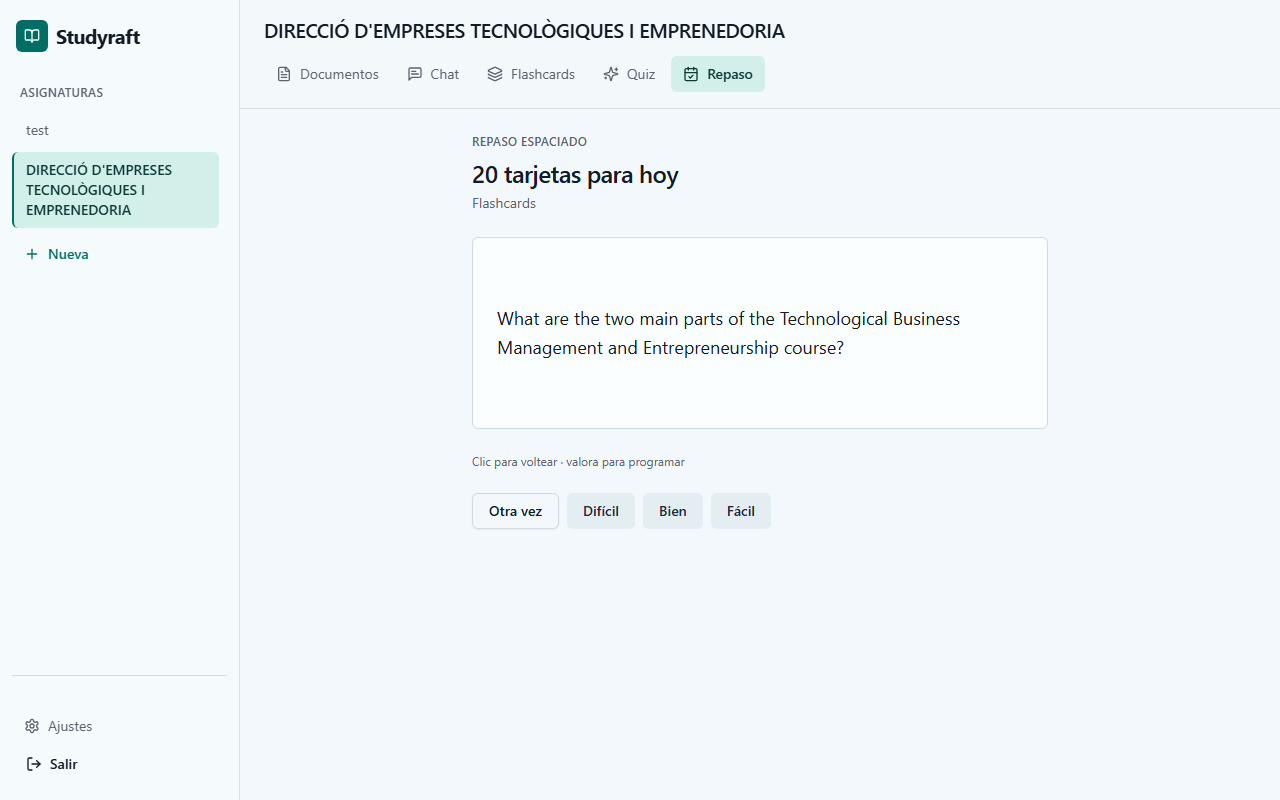
\includegraphics[width=0.92\textwidth]{figures/screenshots/08-planner.png}
\caption{Planner SM-2: targetes pendents d'avui i valoració de qualitat (RF-10).}
\label{fig:ui-planner}
\end{figure}

El qüestionari (figura~\ref{fig:ui-quiz}) es genera sobre el mateix índex; l'ítem visible pregunta el propòsit del BMC «según el documento». El planner (figura~\ref{fig:ui-planner}) mostra la cua del dia i els quatre botons SM-2 de la secció d'exemple numèric (capítol~\ref{cap:desarrollo}). Ni el quiz ni el planner tenen mètrica de qualitat pedagògica en aquest capítol.

\section{Amenaces a la validesa}

En experimentació, una \emph{amenaça a la validesa} és un motiu pel qual la mesura no vol dir el que sembla:

\begin{itemize}
  \item \textbf{Interna.} Un sol corpus i l'autor com a operador del CLI; no hi ha anotació cega de rellevància.
  \item \textbf{Externa.} Apunts d'una assignatura no representen tots els PDF (columnes, escanejos). El corpus és majoritàriament en anglès; les vuit consultes del CLI són en castellà i part de les cartes generades també surten en anglès: l'idioma no està controlat com a factor.
  \item \textbf{Constructe.} La latència de retrieval no és qualitat d'aprenentatge: un sistema ràpid pot citar el fragment equivocat. Les vuit consultes del CLI són factuals; no mesuren resum ni capítol.
  \item \textbf{Fiabilitat.} Les APIs d'LLM no són deterministes. El p50 d'híbrid depèn sobretot d'embeddings i Postgres; el del rerank, del LLM. La primera consulta infla el \texttt{max}.
\end{itemize}

\section{Limitacions observades al producte}

Cites amb snippet, no visor PDF. Agentic d'una sola reescriptura. El pipeline debug relança prerrequisits, no rehidrata artefactes intermedis persistits. La ingestió d'escanejos falla (esperat: PyPDF sense OCR). No s'ha cronometrat l'ingestió ni el xat extrem a extrem. Aquests límits es reprenen com a treball futur, no com a defectes ocults.
